\chapter{Programowanie mikrokontrolerów ARM}

\section{Używanie bibliotek Linux'a}

\section{Środowisko programowania}
Kod programu oraz obsługi stacji pogody, zaimplementowanej na mikrokontrolerze BeagleBone black, został napisany przy użyciu środowiska programistycznego Eclipse. Środowisko to zostało wybreane przez wzgląd na ogromne możliwości, które ułatwiają w znacznej mierze programowanie oraz skracają jego czas. Eclipse jest darmowym narzędziem do programowania, jest intuicyjny w obsłudze, a przede wszystkim posiada wielką rzeszę użytkowników, przez co w przypadku problemów, ich rozwiązanie jest niemal natychmiastowe. Środowisko to można pobrać z oficjalnej strony, w projekcie został wykorzystany \emph{Eclipse IDE for C/C++ Developers}.

\begin{figure}[h]
\centering
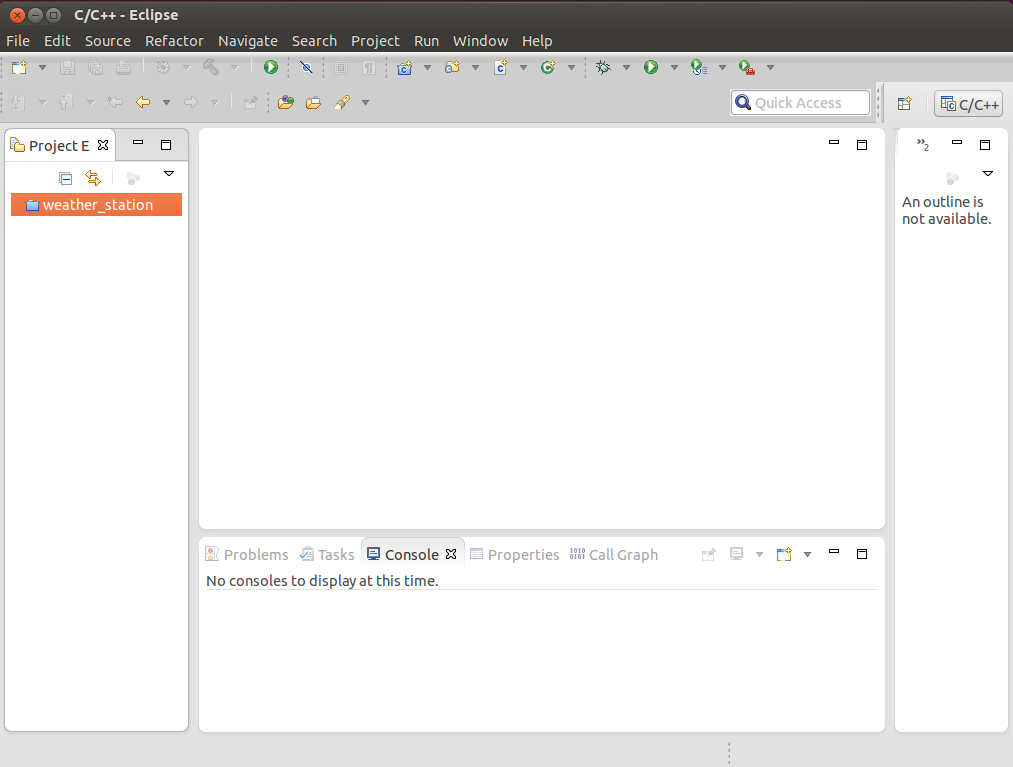
\includegraphics[scale=0.36]{eclipse}
\caption{Główny wygląd Eclipse'a}
\label{fig:eclipse}
\end{figure}

Po rozpakowaniu gotowego środowiska oraz jego uruchomieniu można już zacząć pracę z mikrokontrolerem, wystarczy jeszcze dokonać parę zabiegów, aby czas od zbudowania projektu, do jego uruchomienia na BeagleBone'ie była krótki. W celu uzyskania jak najwygodniejszej konfiguracji, został uruchomiony Eclipse na systemie operacyjnym Ubuntu, na którym były przechowywane wszystkie źródła. Dzięki odpowiedniemu dodatkowi do Eclipse'a - Remote System Explorer istnieje możliwość tworzenia programu na komputerze, jego cross-kompilacji do aplikacji wykonywalnej oraz uruchomienia gotowego pliku binarnego na mikrokontrolerze. Dzieje się to dzięki wspomnianemu wcześniej protokołowi SSH.

Aby stworzyć nowy projekt należy kliknąć File->New->C Project (może być również C++), pojawi się następujące okno:

\begin{figure}[h]
\centering
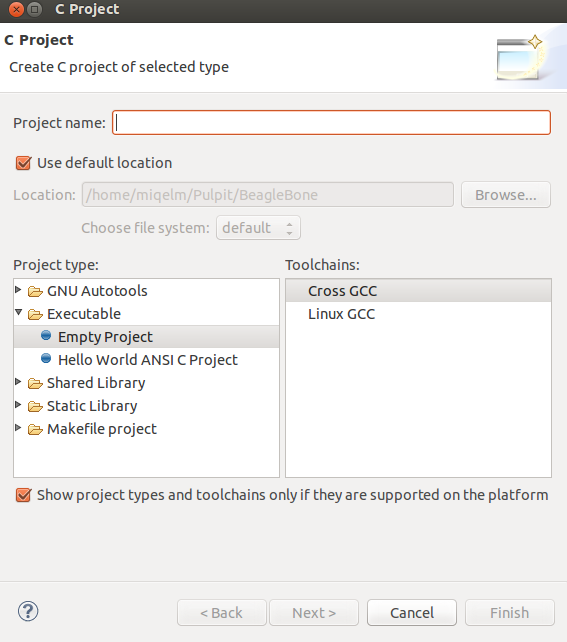
\includegraphics[scale=0.36]{eclipse_new}
\caption{Tworzenie nowego projektu}
\label{fig:eclipse_new}
\end{figure}

Po uzupełnieniu nazwy projektu oraz wyboru Cross GCC, przechodzimy dalej i kończymy konfigurację. Teraz następuje najważniejsza rzecz. Aby skompilować nasz projekt i móc go uruchomić na innej platformie sprzętowej, jaką jest procesor ARM, potrzebujemy cross-kompilatora. Jest to wymagane, gdyś komputer oraz BeagleBone różnią się budową oraz sposobem komunikacji na najniższym poziomie. W związku z tym, należy na komputerze zainstalować narzędzie umożliwiające nam generowanie pliku binarnego na inną platformę sprzętową, proces ten jest nazywany cross-kompilacją.

BeagleBone Black jest wyposażony w procesor o architekturze ARM hard float, dlatego też potrzebujemy do niego kompilatora, nazywa się on arm-linux-gnueabihf-gcc. Aby go zainstalować, należy w konsoli użytkownika wpisać następującą komendę:\newline
\emph{sudo apt-get install arm-linux-gnueabihf-gcc}\newline
Potwierdzająć chęć zainstalowania oraz pomyślnym przebiegu instalacji, jesteśmy w stanie teraz skompilować program na architekturę ARM.

W Eclipse klikając teraz prawym przyciskiem myszy na nowo stworzony projekcie, następnie wciśnięciu Properties, ukazują nam się właściwości projektu. Należy teraz zakomunikować środowisku, że program będzie kompilowany przy użyciu zainstalowanego przed chwilą kompilatora. W tym celu należy uruchomić zakładkę C/C++ Build, a potem opcję Settings i Cross GCC Compiler, w polu Command należy wpisać nazwę cross-kompilatora. Poniżej zostaje zamieszczony zrzut ekranu przedstawiający zaistniałą sytuację:

\begin{figure}[h]
\centering
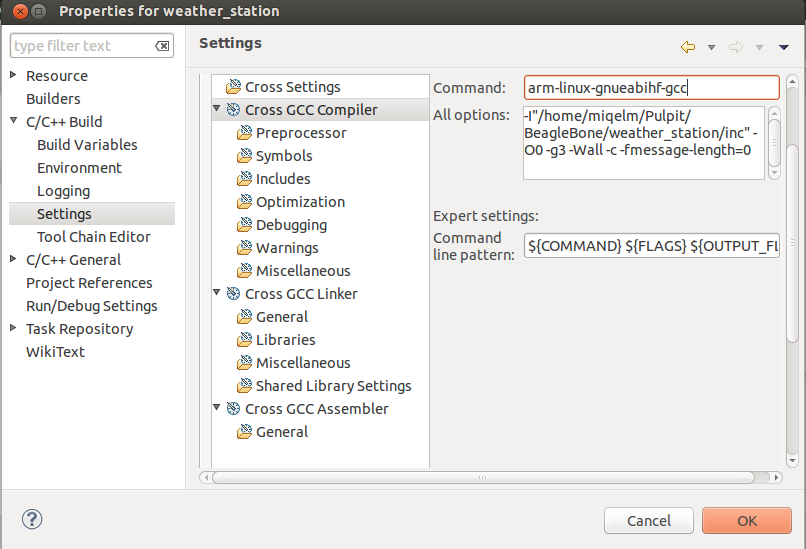
\includegraphics[scale=0.36]{eclipse-settings}
\caption{Ustawienia projektu}
\label{fig:eclipse-settings}
\end{figure}

W podobny sposób należy wypełnić również pola Command w zakładkach Cross GCC Linker oraz Cross GCC Assembler, ten ostatni należy wypełnić wpisując: arm-linux-gnueabihf-as.

\section{Kompilator}